\documentclass[10pt]{article}

\usepackage[utf8]{inputenc}
\usepackage[francais]{babel}
\usepackage{multicol}
\usepackage{float}
\usepackage{tikz}

% FAMFAMFAM.com colors
\definecolor{mpink}{RGB}{255,11,91}
\definecolor{mblue}{RGB}{11,206,255}
\definecolor{mgreen}{RGB}{123,255,45}

\setlength{\textwidth}{39pc}
\setlength{\textheight}{50pc}
\setlength{\parindent}{1em}
\setlength{\parskip}{0pt plus 1pt}
\setlength{\oddsidemargin}{0pc}
\setlength{\marginparwidth}{0pc}
\setlength{\topmargin}{1pc}
\setlength{\headsep}{20pt}
\setlength{\columnsep}{2pc}

\title{Recherche décentralisée de connexité pour réseaux de capteurs mobiles}
\author{Merwan Achibet}
\date{}

\begin{document}

\maketitle

\begin{multicols}{2}

\section{Introduction}

On imagine le problème suivant : un groupe de $n$ capteurs mobiles est
réparti aléatoirement dans un espace aérien. On part de l'hypothèse
qu'un capteur connaît uniquement le nombre total de capteurs de ce
système et qu'il est assez sophistiqué pour pouvoir déterminer
précisément sa position absolue. Les capteurs sont dotés de matériel
de communication sans fil et peuvent s'envoyer des messages à
condition que la distance les séparant soit inférieure à leur rayon
d'émission $R_c$.

Le réseau constitué par cet essaim d'appareils volants forme un graphe
dynamique dont les n\oe uds sont les capteurs. Deux n\oe uds sont
reliés par un arc si les capteurs qui leur sont associés sont en
mesure de communiquer, id est s'ils sont assez proches. La figure
\ref{communication} décrit un exemple de scénario impliquant trois
capteurs.

\begin{figure}[H]

  \centering

  \begin{tikzpicture}

  \draw (0,0) -- (-1,1);

  \drawSensor{0}{0}{2}{red}
  \drawSensor{-1}{1}{2}{blue}
  \drawSensor{2.5}{1}{2}{green}

\end{tikzpicture}


  \caption{Les capteurs rose et bleu peuvent communiquer et sont
    connectés tandis que le capteur vert est isolé.}
  \label{communication}

\end{figure}

On considère un capteur comme un agent autonome capable de se mouvoir
dans l'espace. Afin de ne pas se préoccuper de considérations
géométriques superflues, il est supposé qu'un capteur conserve
toujours la même altitude et donc on limite son déplacement à deux
dimensions. La contrainte principale de cet exercice est que l'on
refuse toute forme de contrôle global sur l'essaim de capteurs. Toutes
les actions entreprises par un appareil seront uniquement dû à ses
décisions propres; décisions dépendants de la vue réduite du système
dont il dispose.

La possibilité pour un capteur de communiquer avec ses semblables est
au centre de nos préoccupations car on considère qu'un capteur isolé
est inutile puiqu'incapable de partager des données. Dans le contexte
de l'étude décentralisée d'un graphe dynamique, deux questions se
posent :

\begin{enumerate}
\item{Comment déterminer si le réseau de capteurs est connexe ?}
\item{Comment déplacer les capteurs de façon à ce qu'il le devienne ?}
\end{enumerate}

Pour répondre à la première question, on se concentrera sur les
communications de capteur à capteur en proposant une méthode pour
laquelle chaque agent diffuse sa vision de la connexité du réseau,
étiquettée en fonction de l'origine de l'information et de sa date. Un
mécanisme de filtrage autorégulant sera mis en place pour
répandre rapidement les informations critiques telles que l'ajout d'un
nouveau n\oe ud à une composante connexe ou la disparation d'un autre.

La réponse à la seconde question s'attachera à l'aspect mobile d'un
capteur. On proposera un guidage décentralisé se basant sur
l'imitation de plusieurs lois physiques de la nature afin de former un
maillage à la fois connexe, équilibré et étalé dans
l'espace. Finalement, on envisagera une extension de ce système pour
permettre aux capteurs d'éviter naturellement les obstacles.

\section{Déterminer si le réseau est connexe}

Le réseau de capteur est hautement dynamique. Sa connexité dépend du
mouvement des capteurs et de leur état de fonctionnement

Une étiquette correspond à une information de connexité, relayée de
capteur en capteur. Son information principale est le n\oe ud du
réseau qu'elle concerne mais elle comprend aussi la date à laquelle
l'information est entrée dans le système et le n\oe ud à son origine.

Si l'on traduisait le message d'un capteur à un autre en langue
humaine, on pourrait entendre Bonjour, je suis le capteur D, selon moi
A et B sont connectés et j'ai des doutes sur F

Un message contient deux listes

\begin{itemize}
\item{La liste des n\oe uds dont on est certain qu'ils appartiennent
  au réseau}
\item{La liste des n\oe uds en situation douteuse}
\end{itemize}

\section{Rendre le réseau connexe}

La résolution de ce problème passe par la satisfaction de deux besoins
a priori antagonistes. D'une part, il est naturellement nécessaire de
réunir les capteurs dans un espace réduit, de façon à ce qu'ils
puissent communiquer et échanger des données en continu. D'autre part,
et dans l'interêt de leurs utilisateurs, ils doivent s'étaler dans
l'espace afin d'effectuer des mesures sur la plus grande superficie
possible. Nous sommes donc dans une situation de compromis, dans
laquelle une contrainte technique (la portée de communication) force à
agglomérer les capteurs en une même zone, tandis que leur but premier
est de ramasser des données en masse et donc, rationnellement, de
s'éloigner les uns des autres pour couvrir le plus de terrain
possible. La seule issue favorable à ce problème est donc d'aboutir à
une situation d'équilibre satisfaisant ces deux contraintes
diamétralement opposées.

Le cadre de cet exercice s'accorde parfaitement avec la problèmatique
de la prise de décision dans un réseau décentralisé puisque chaque
capteur peut être assimilé à un agent autonome, capable d'agir sur la
configuration de son environnement en se déplaçant dans l'espace. Quel
que soit l'état d'un capteur, la vision du système dont il dispose est
locale et doit servir seule à déterminer quelles actions il
entreprend. L'objectif est donc ici de proposer une méthode de guidage
que chaque capteur peut adopter et qui, par émergence d'une dynamique
globale, résoudra notre problème en répartissant les capteurs dans
l'espace de façon satisfaisante.

Les boïds de Craig Reynolds \cite{Reynolds1987} sont reconnus pour
simuler un comportement de groupe a priori complexe et synchronisé à
partir d'un jeu de règles simples. On s'en inspire, ainsi que d'un
modèle de mouvement particulaire \cite{Cheng2011497} se basant sur la
répulsion entre molécules de gaz, pour concevoir les trois règles qui
gouverneront notre système. Chacune de ces lois, que l'on présente
séparément par la suite, va engendrer une influence sur le déplacement
de nos capteurs; influence dont la composition sera détaillée en
dernière partie.

\subsection{Attraction}

\`A la lecture de l'énoncé de ce problème, la nécessité de rapprocher
les capteurs les uns des autres, afin qu'un réseau de communication
ininterrompu se forme, vient naturellement à l'esprit. En effet, la
condition \textit{sine qua non} au bon fonctionnement du réseau est la
communication. Un capteur isolé est inutile puisque son
information n'est pas partagée.

Par sa loi de la gravitation universelle, Isaac Newton décrit la force
qui attire toute paire de corps comme étant proportionnelle à leur
masse respective et à la distance les séparant. Nous nous permettons
de simplifier quelque peu son équation et d'en retirer l'aspect
massique pour obtenir une règle qui a tout couple de corps associe une
attraction proportionnelle à leur distance. S'ils obéissaient à cette
loi, nos capteurs auraient naturellement tendance à se grouper, et
donc à se mettre à portée de communication les uns des autres.

\`A l'échelle de notre système, le cadre est différent de celui de la
loi de Newtion, et cette influence n'est pas universelle. Nous ne
pouvons malheureusement pas réécrire les règles de ce monde et
inventer une attirance magique entre toute paire de capteurs. On peut
néanmoins la simuler. Si deux capteurs sont à portée et peuvent
échanger leur positions respectives alors la détermination de la
distance les séparant est aisée. \`A partir de là, on peut imiter un
phénomène d'attration.

Concrètement, on associe à tout capteur $c$ un rayon d'attraction
$R_a$ (voir figure \ref{attraction}). Si un capteur voisin se trouve à
la fois dans le rayon de communication $R_c$ de $c$ et à l'extérieur
de $R_a$, la force d'attraction que ce capteur devra subir est fournie
par la formule suivante :

$$
\vec{a} = \frac{\vec{p}_c - \vec{p}_v}{|\vec{p}_c - \vec{p}_v|^2}
$$

\begin{figure}[H]

  \centering

  \begin{tikzpicture}

  \drawSensor{0}{0}{2}{black}
  \draw (0,0) circle (1.5);

  \draw[fill=black] (200:1.8) circle (0.1);
  \draw[->] (200:1.8) -- (200:1);

\end{tikzpicture}


  \caption{En vert, le rayon d'attraction, dont l'intensité est
    décroissante de l'extérieur vers l'intérieur.}
  \label{attraction}

\end{figure}

On note que l'attraction n'a pas pour but d'approcher des capteurs
trop éloignés pour communiquer puisque l'existence d'une connexion
entre deux capteurs est un prérequis à l'application de la force
d'attraction. ???

Dans le phénomène d'attraction réel, l'action est réciproque et
instantanée mais dans notre cas elle est unidirectionnelle. Un capteur
est attiré par tous ses voisins mais le processus décrit ne modifie
pas directement la position du voisin et il n'en subit aucune
influence. Il est néanmoins à prévoir que lorsque ce voisin calculera
les influences qui s'appliquent à lui, il en subira la réciproque.

\subsection{Répulsion}

L'attraction a pour effet d'agglomérer en groupes serrés tous les
capteurs démarrant la simulation dans une même zone. Mais même si de
cette façon la communication est assurée, les capteurs finissent par
tous être superposés sur la même position au bout d'un certain nombre
d'itérations et la contrainte de couverture n'est absolument pas
satisfaite.

Pour pallier cette déconvenue, on introduit une nouvelle force opposée
à l'attraction, la répulsion. Le rayon $R_r$ définit une nouvelle zone
radiale qui, contrairement à la loi précédente, expulsera les capteurs
envahissants vers l'extérieur. Il est bien sûr nécessaire que $R_r <
R_c$.

$$
\vec{r} = (\vec{p} - \vec{p_v}) ???
$$

\begin{figure}[H]

  \centering

  \begin{tikzpicture}

  \drawSensor{0}{0}{2}{black}
  \draw (0,0) circle (1.5);

  \draw[fill=black] (150:0.5) circle (0.1);
  \draw[->] (150:0.5) -- (150:1.3);

\end{tikzpicture}


  \caption{En rouge, le rayon de répulsion, dont l'intensité est
    décroissance du centre vers les bords.}
  \label{repulsion}

\end{figure}

On prend $R_r = R_a - \varepsilon$, o\`u $\varepsilon$ correspond à la
largeur d'une bande neutre entourant chaque capteur (voir figure
\ref{repulsion}). Les capteurs auront naturellement tendance à
s'installer dans ces zones libre de toute influence et à se verouiller
???. Nous verrons par la pratique que la conséquence principale de ce
positionnement forcé est un maillage régulier et géométrique. La
régularité spatiale du réseau de capteur est ici un bonus
appréciable. ???

\subsection{Gravité}

Les deux règles présentées permettant aux capteurs proches de
s'agglomérer en composantes connexes équilibrées mais notre objectif
est d'obtenir une unique composante connexe. Dans cette optique, on
introduit une dernière influence inspirée du physique, la gravité.

Comme spécifié en introduction, on part de l'hypothèse que les
capteurs sont munis de moyens de localisation dans l'espace et nous en
avons allègrement profiter pour les calculs de distances des formules
précédentes. Toujours dans cette ???, on peut supposer que tous les
capteurs connaissent le centre de l'environnement dans lequel ils sont
largués. Cette position peut être la position de laquelle ils ont été
largués, une position pré-programmée ou un point calculée de façon
commune par moyenne de toutes leur position(sujet intéréssant
!). L'important est que cette position soit connu de tous et servent
d'origine dans leur repère.

La gravité est la force qui va attirer tous les capteurs vers le
centre de l'environnement. \`A première vue, une telle règle semble
dangereuse car on imagine qu'elle forcera les capteurs à se déplacer
vers le centre de leur environnement au risque de sacrifier la
couverture dont nous fait disposer l'effet répulsif
inter-particulaire. Néanmoins, on compte sur l'effet combiné des
différentes forces pour résister à cet effet.

Son intérêt est d'amener vers le centre les composantes connexes et
les capteurs isolés pour tous les assembler en un unique réseau.

$$
\vec{g} = -\vec{p} ???
$$

\begin{figure}[H]

  \centering

  \begin{tikzpicture}

  \node[path picture={
      \draw[black] (path picture bounding box.south east) -- (path
      picture bounding box.north west);
      \draw[black] (path picture bounding box.north east) -- (path
      picture bounding box.south west);}] at (0,0) {};

  \draw[fill=black] (120:3) circle (0.1);
  \draw[->] (120:3) -- (120:2.5);

  \draw[fill=black] (180:3) circle (0.1);
  \draw[->] (180:3) -- (180:2.5);

  \draw[fill=black] (10:3) circle (0.1);
  \draw[->] (10:3) -- (10:2.5);

\end{tikzpicture}


  \caption{La gravité attire tous les capteurs vers le centre de leur
    environnement.}
  \label{gravite}

\end{figure}

\subsection{Composition d'une force nette}

Une fois ces trois forces calculées, on ne peut pas les appliquer
naïvement sur le capteur concerné car il s'agit d'un objet physique
soumis à des limitations quant à sa vitesse de déplacement. On associe
donc à chaque capteur une vitesse de déplacement maximale qui servira
de borne supérieure à la magnitude des trois forces combinées.

Puisque l'on dispose de trois influences différentes, chacune tenant
un rôle particulier dans la résolution du problème, l'idée la plus
intuitive est d'en déduire une influence moyenne.

$$
\vec{f} = \frac{\vec{a} + \vec{r} + \vec{g}}{3}
$$

En pratique, on observe que ce choix montre vite ses limites. Dans
certains cas, deux forces seront opposées et par ce type de
combinaison, elles s'annulleront mutuellement et on obtiendra au final
un mouvement nul. Et l'immobilité n'est pas une solution envisageable
à ce problème. Dans d'autre cas encore plus fréquents, les trois
forces semblents adaptées : on observe des capteurs éparses flotter
lentement vers le centre de leur environnement et s'assembler en
composante connexe de plus en plus grande au fur et à mesure de leur
traversée de l'espace. Mais une fois que le maillage est complet et
qu'une situation d'équilibre semble avoir été atteinte, le centre du
réseau commence à trembler, les capteurs se rapprochent dangereusement
et force le passage vers le centre en ignorant les rayons de
répulsions de leur voisin. Ce problème est dû au nombre elevé de
tensions s'opérant au centre du réseau, résultant en une pression
intense qui fait s'effondrer le réseau jusqu'à ce que tous les
capteurs occupent la même position. Moyenner les forces est donc une
fausse bonne idée.

MEILLEURE SOLUTION

DEMO EN TROIS IMAGES

\subsection{Obstacles}

On propose d'étendre ce modèle de guidage afin de permettre aux
capteurs d'éviter automatiquement les obstacles par l'ajout d'une
nouvelle force virtuelle. Ici, un obstacle est défini comme étant une
zone non traversable. En réalité, il peut s'agir d'un bâtiment, d'une
zone dont les relevés ne nous intéressent pas, ou d'une zone interdite
au appareils volants.

REPULSION

\begin{figure}[H]

  \centering

  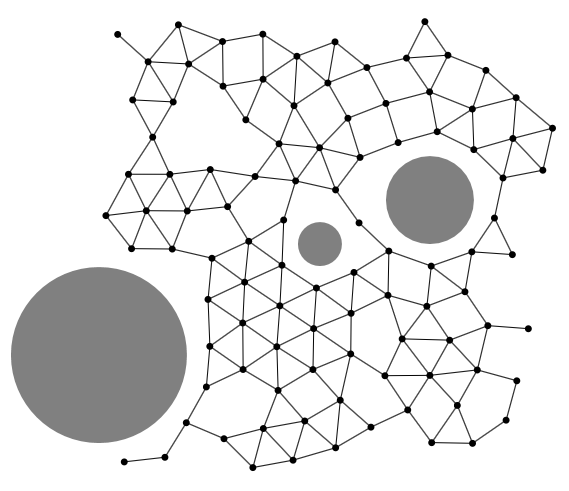
\includegraphics[width=7cm]{obstacles.png}

  \caption{}
  \label{obstacles}

\end{figure}

\section{Conclusion}



\end{multicols}

\bibliographystyle{alpha}
\bibliography{references}

\end{document}
